\documentclass[titlepage, a4paper]{article}
\usepackage[english]{babel}
\usepackage[utf8]{inputenc}
\usepackage{graphicx}
\usepackage{color}
\usepackage{mathtools}
\usepackage{float}
\usepackage[parfill]{parskip}
\usepackage[margin=10pt,font=small,labelfont=bf,labelsep=endash]{caption}
\usepackage{epstopdf}
\usepackage{listings}
\usepackage{enumitem}
\epstopdfsetup{suffix=}
\DeclareGraphicsExtensions{.ps}
\DeclareGraphicsRule{.ps}{pdf}{.pdf}{`ps2pdf -dEPSCrop -dNOSAFER #1 \noexpand\OutputFile}

\lstset{literate=%
    {å}{{\r{a}}}1
    {ä}{{\"a}}1
    {ö}{{\"o}}1
    {Å}{{\r{A}}}1
    {Ä}{{\"A}}1
    {Ö}{{\"O}}1
}

\newcommand{\todo}[1] {\textbf{\textcolor{red}{#1}}}

\usepackage{fancyhdr}
\fancyhead[L]{}
\pagestyle{fancy}
\rhead{Pål Kastman \\ Alexander Yngve}
\chead{TDTS08}
\thispagestyle{empty}

\begin{document}

{\ }\vspace{45mm}

\begin{center}
  \Huge \textbf{TDTS08: whattolearn}
\end{center}

\vspace{250pt}

\begin{center}
  \begin{tabular}{|*{3}{p{40mm}|}}
    \hline
    \textbf{Name} & \textbf{PIN} & \textbf{Email} \\ \hline
           {Pål Kastman} & {851212-7575} & {palka285@student.liu.se} \\ \hline
           {Alexander Yngve} & {930320-6651} & {aleyn573@student.liu.se} \\ \hline
  \end{tabular}
\end{center}
\newpage

\tableofcontents
\thispagestyle{empty}
\newpage

\section{Introduction}
This documents only purpose is to document what I will need to learn in the course tdts08. \\
\todo{YNGVE OM DU VILL BYTA RUBRIKERNA SÅ ÄR DET HELT OKEJ, DOM ÄR BARA DÄR SOM STÖD NU}

\section{Lecture 2: Memory Systems}

\textbf{Sequential access}: Memory is organized into units of data, called records. Access must be made in a specific linear sequence. Stored addressing information is used to separate records and assist in the retrieval process. A shared read–write mechanism is used, and this must be moved from its current location to the desired location, passing an rejecting each intermediate record. Thus, the time to access an arbitrary record is highly variable. \textbf{Tape units}  are sequential access.

\textbf{Direct access}: As with sequential access, direct access involves a shared read–write mechanism. However, individual blocks or records have a unique address based on physical location. Access is accomplished by direct access to reach a general vicinity plus sequential searching, counting, or waiting to reach the final location. Again, access time is variable. \textbf{Disk units} are direct access.

\textbf{Random access}: Eacha ddressable location inm emory has a unique, physically wired-in addressing mechanism. The time to access a given location is inde- pendent of the sequence of prior accesses and is constant. Thus, any location can be selected at random and directly addressed and accessed. Main memory and some cache systems are random access.

\textbf{Associative}: This is arandom access type of memory that enables one to make a comparison of desired bit locations within a word for a specified match, and to do this for all words simultaneously. Thus, a word is retrieved based on a portion of its contents rather than its address.

\textbf{Access time (latency)}: For random-access memory, this is the time it takes to perform a read or write operation, that is, the time from the instant that an address is presented to the memory to the instant that data have been stored or made available for use. For non-random-access memory, access time is the time it takes to position the read–write mechanism at the desired location.

\textbf{Transfer rate}: This is the rate at which data can be transferred into or out of a memory unit. For random-access memory, it is equal to 1/(cycle time).
For non-random-access memory, the following relationship holds:

$$T_n = T_A + \frac{n}{R}$$

$T_n$ = Average time to read or write n bits \\
$T_A$ = Average access time \\
$n$ = Number of bits \\
$R$ = Transfer rate, in bits per second (bps) \\

\subsection{Memory hierarchy}
\textbf{Registers} Built into the processors, very small and expensive. \\
\textbf{Main Memory} Memory that the cache collects data from. \\
\textbf{Secondary Memory (of direct access type)} Bigger in size, but less expensive per Byte. \\
\textbf{Secondary Memory (of archive type)} And so on. \\



\subsection{Cache memory}
There is a big gap in speed between register and main memory, this is why we need to use cache memory.

Cache memory is designed to combine the memory access time of expensive, high-speed memory combined with the large memory size of less expensive, lower-speed memory.
ller, faster cache memory.

The cache contains a copy of portions of main memory. When the processor attempts to read a word of memory, a check is made to determine if the word is in the cache. If so, the word is delivered to the processor. If not, a block of main memory, consisting of some fixed number of words, is read into the cache and then the word is delivered to the processor.

We would like the size of the cache to be small enough so that the overall average cost per bit is close to that of main memory alone and large enough so that the overall average access time is close to that of the cache alone.




\subsubsection{Locality of reference}
The intermediate-future memory access will usually refer to the same word or words in the neighborhood, and will not have to involve the main memory.

\textbf{Temporal Locality} -- If an item is referenced, it will tend to be referenced again in the near future. \\
\textbf{Spatial Locality} -- If an item is referenced, items whose addresses are close by will tend to be referenced soon. \\

\subsubsection{Replacement methods}
yes, there's different kinds of them.

\subsubsection{Cache Design}

One, two, three level caches, how does it work. up- and downsides of them.

\textbf{Split Caches} means that we have separate caches for instructions and data. \\
+ Competition for the cache between instruction and data is eliminated \\
+ Instruction fetch can proceed in parallel with memory access from the CPU for operands. \\
- One may be overloaded while the other is under utilized. \\

\textbf{Unified Caches} means that both instructions and data uses the same cache.
+ Better balance the load between instruction and data fetches depending on the dynamics of the program execution. \\
+ Design and implementation are cheaper. \\
-- Lower performance. \\
\subsubsection{Direct mapping cache}
Each block of the main memory is mapped into a fixed cache slot. \\
+ Simple to implement and therefore inexpensive. \\
-- If a program accesses 2 blocks that map to the same cache slot repeatedly, cache miss rate is very high. \\

\subsubsection{Associative mapping cache}
A main memory block can be loaded into any slot of the cache. To determine if a block is in the cache, a mechanism is needed to simultaneously examine every slot’s tag. In this case, the cache control logic interprets a memory address simply as a Tag and a Word field. The Tag field uniquely identifies a block of main memory. To determine whether a block is in the cache, the cache control logic must simultaneously examine every line’s tag for a match. \\

The downside of this is the complex circuitry needed to examine all the tags.

\subsubsection{Set Associative mapping cache}
A fully associative mapped memory can be built but is very expensive, and therefore is not done. Instead we use a \textbf{set associative} cache memory. \\
Here the cache are divided into a number of sets, where each set contains a number of slots (just like a regular cache). 


\subsubsection{Fully Associative Organization}


\subsubsection{Write Policy}
When a block in the cache is to be replaced, we have to consider two cases. If the block in the case has \textbf{not been altered}, then it can be replaced with a new block without saving the block to the main memory. Or if it \textbf{has been altered} (one block is enough), then we need to write that block back to main memory. \\

There are two cases to consider
\begin{enumerate}
\item More than one device may have access to main memory. \\
  
  For example, an I/O module may be able to read-write directly to memory. If a word has been altered only in the cache, then the corresponding memory word is invalid. Further, if the I/O device has altered main memory, then the cache word is invalid. \\
\item Multiple processors are attached to the same bus and each processor has its own local cache. Then, if a word is altered in one cache, it could conceivably invalidate a word in other caches.
\end{enumerate}
\textbf{Write through} all write operations are made to main memory as well as to the cache, ensuring that main memory is always valid. Any other processor–cache module can monitor traffic to main memory to maintain consistency within its own cache. The main disadvantage of this technique is that it generates substantial memory traffic and may create a bottleneck.\\

\textbf{Write through with buffered write} The same as write-through, but instead of slowing the processor down by writing directly to main memory, the write address and data
are stored in a high-speed write buffer; the write buffer transfers data to main memory while the processor continues its task.\\

\textbf{Write back} With write back, updates are made only in the cache. When an update occurs, a dirty bit, or use bit, associated with the line is set. Then, when a block is replaced, it is written back to main memory if and only if the dirty bit is set. \\

\subsection{Virtual memory}
Almost all nonembedded processors, and many embedded processors, support virtual memory. In essence, virtual memory is a facility that allows programs to address memory from a logical point of view, without regard to the amount of main memory physically available. When virtual memory is used, the address fields of machine instructions contain virtual addresses. For reads to and writes from main memory, a hardware memory management unit (MMU) translates each virtual address into a physical address in main memory.

\subsubsection{Paging}
Unequal fixed-size and variable-sized partitions of memory are inefficient, we need to make sure that we use the most of the memory available in the best way, we try to do this using pages.

We first divide programs into fixed sized memory blocks called pages, then we divide the main memory into equal fixed sized blocks, called page frames. \\

A process then needs a set of free page frames assigned by the OS. Then its up to the OS to make sure it keeps track of the free available frames, it also uses a page table to keep track of the mapping between pages and page frames. 

\subsubsection{Page fault}
When we try to access a piece of memory that is not currently in the main memory, but instead in the virtual memory. The OS must then load the page into the main memory firs, this is called a \textbf{Page fault}.

\subsubsection{Page replacement}
When a page fault occurs and all the page frames are occupied, one of them must be replaced. If the page that are to be replaced, has been modified, we need to write that memory back to the secondary storage. \\

We want to replace a page that we think will not be accessed for the longest amount of time. The problem is that we can't predict the future, so we have to predict the future, we can do this in some different ways, described below.

\subsubsection{Replacement algorithms}
Not needed with direct mapping, but with associative mapping we need one of these algorithms. \\

\textbf{First-in-first-out} \\
\textbf{Least recently used (LRU)}: replaces the cache that has been in the cache the longest without being referenced.\\
\textbf{Least frequently used (LFU)}: replaces the cache that has been referenced the least frequent.\\ 
\textbf{Random}\\ 

\section{Lecture 3: Instruction pipelining}
The idea is to divide the workload into different stages, so that we don't have to wait for an instruction to complete before we fetch the next one.

The typical pipeline has \textbf{six} stages: \\
1. Fetch Instruction (FI): Fetch the instruction.\\
2. Decode Instruction (DI): Determine the op-code and the operand specifiers.\\
3. Calculate Operands (CO): Calculate the effective addresses.\\
4. Fetch Operands (FO): Fetch the operands.\\
5. Execute Instruction (EI): perform the operation.\\
6. Write Operand (WO): store the result in memory.\\

The ideal case gives us a speed-up of six times. But in practice we have some problems.

In general, a larger number of stages gives better performance. \\
However, a large number also increases the complexity. We have to  move a lot of information between stages, and synchronize the stages. We call the problems that occur \textbf{Pipeline Hazards}.

\subsection{Pipeline hazards}
There are different kinds of pipeline hazards, first we have the case with dependency, A pipeline hazard occurs when the pipeline, or some portion of the pipeline, must stall because conditions do not permit continued execution. Such a pipe- line stall is also referred to as a pipeline bubble. There are three types of hazards: resource, data, and control. \\

\subsubsection{Structural (resource) hazards}
A \textbf{Resource hazards} resource hazard occurs when two (or more) instructions that are already in the pipeline need the same resource. The result is that the instructions must be executed in serial rather than parallel for a portion of the pipeline. A resource hazard is sometime referred to as a structural hazard.

\subsubsection{Data hazards}
A \textbf{Data Hazard} is when two instructions in a program are to be executed in sequence and both access a particular memory or register operand. If the two instructions are executed in strict sequence, no problem occurs. However, if the instructions are executed in a pipeline, then it is possible for the operand value to be updated in such a way as to produce a different result than would occur with strict sequential execution.

There are three types of data hazards: \\
• Read after write (RAW), or true dependency: An instruction modifies a reg- ister or memory location and a succeeding instruction reads the data in that memory or register location. A hazard occurs if the read takes place before the write operation is complete. \\
• Write after read(WAR), or antidependency: Aninstructionreadsaregisteror memory location and a succeeding instruction writes to the location. A hazard occurs if the write operation completes before the read operation takes place. \\
• Write after write (WAW), or output dependency: Two instructions both write to the same location. A hazard occurs if the write operations take place in the reverse order of the intended sequence. \\

We can handle this by using a technique called forwarding (bypassing). This works in the following way: \\
The ALU passes its result back into a MUX. If this detects that the value have been updated and not yet written back into the main memory, the value from the ALU will be used instead of the value we fetched from the memory as can be seen in figure \ref{fig:bypassing}.

\begin{figure}[H]
	\centering
	\scalebox{0.342}{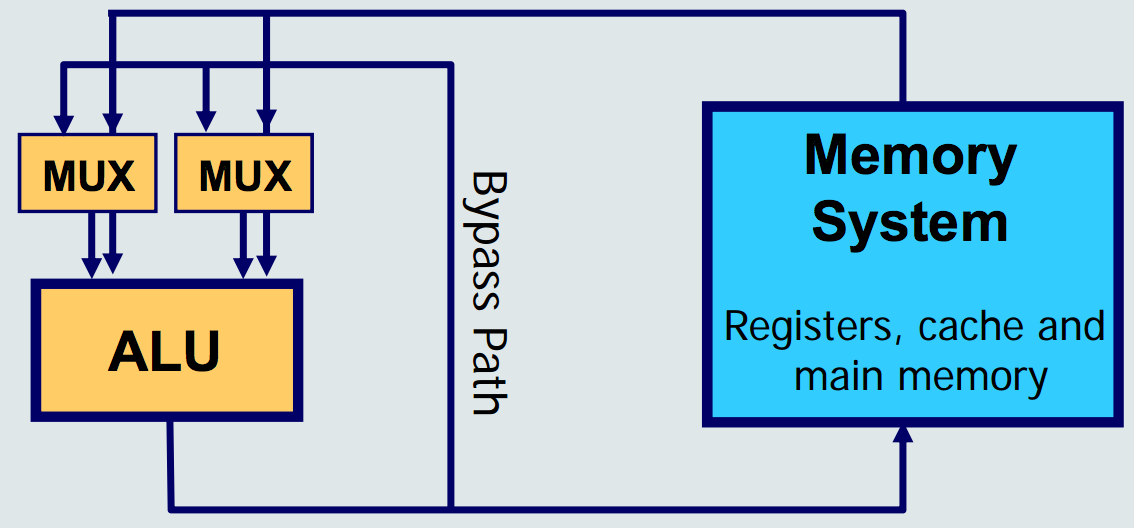
\includegraphics{img/bypassing.png}}
	\caption{The ALU passes its calculated value back into a MUX.}
	\label{fig:bypassing}
\end{figure}

\subsubsection{Control hazards}
A \textbf{control hazard}, also known as a branch hazard, occurs when the pipeline makes the wrong decision on a branch prediction and therefore brings instructions into the pipeline that must subsequently be discarded as seen in figure \ref{fig:control-hazard}.

\begin{figure}[H]
	\centering
	\scalebox{0.342}{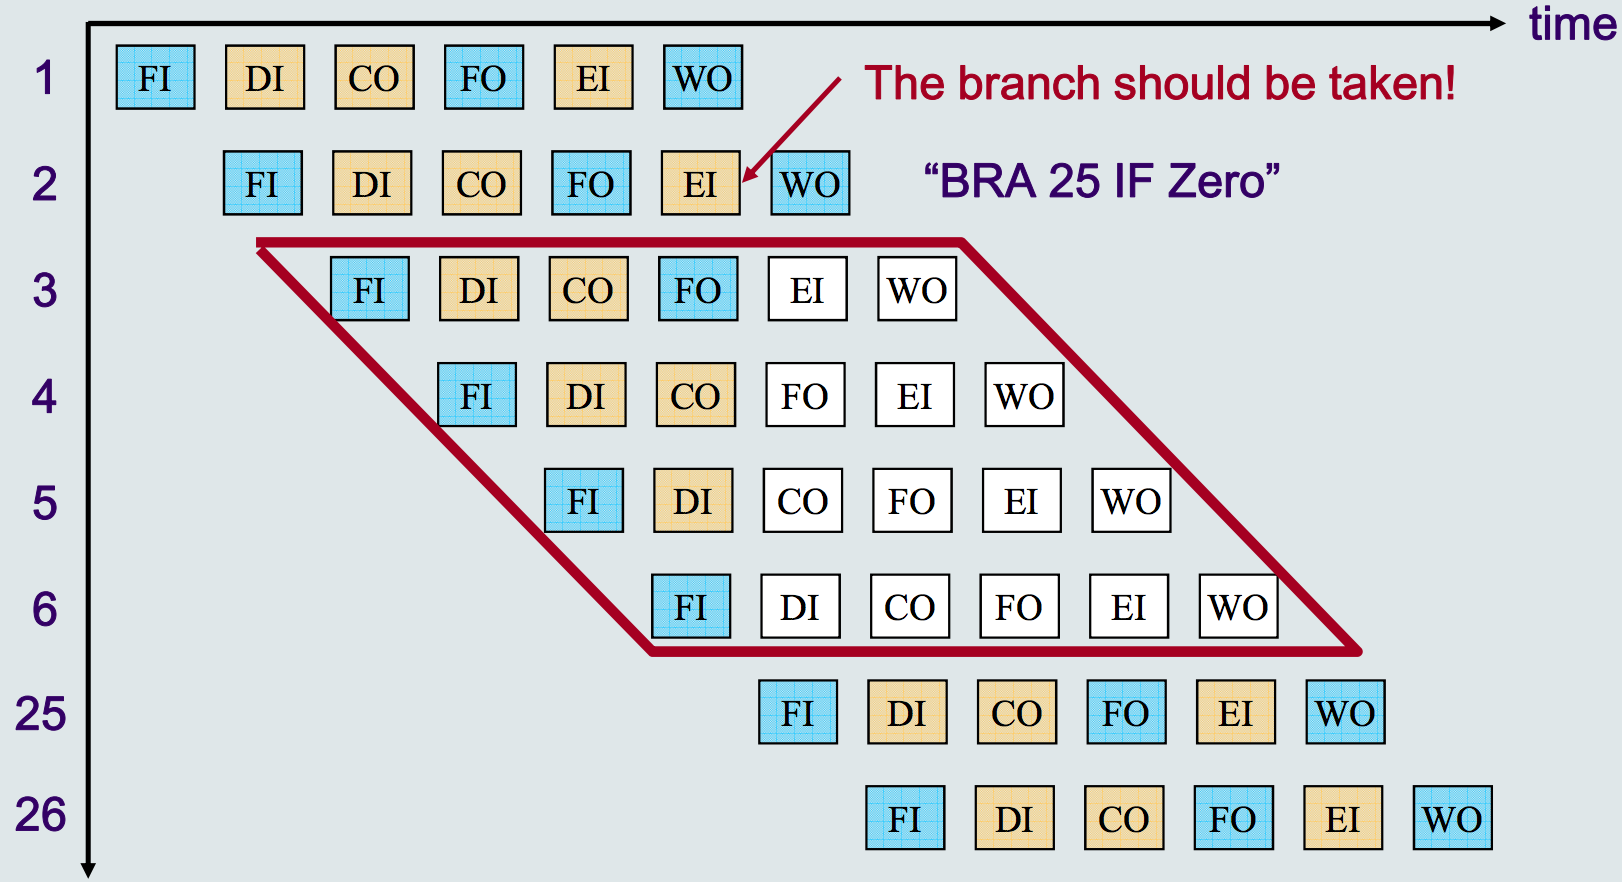
\includegraphics{img/control-hazard.png}}
	\caption{Control hazards.}
	\label{fig:control-hazard}
\end{figure}


\subsection{Branch handling}
There are different ways of handling branches. \\

\subsubsection{Stop the pipeline}
We can stall all the next instructions until the current branch reaches its final stage and we know what to do, this is expensive due to that 20-35\% of the things instructions executed are executed as branches.

\subsubsection{Multiple streams}
Implement hardware resources so that we can execute both alternatives in parallel, there are two problems with this though:
\begin{enumerate}
\item With multiple pipelines there are contention delays for access to the registers and to memory. \\
\item Additional branch instructions may enter the pipeline (either stream) before the original branch decision is resolved. Each such instruction needs an addi- tional stream.
\end{enumerate}

\subsubsection{Pre-fetch branch target}
When a conditional branch is recognized, the target of the branch is prefetched, in addition to the instruction following the branch. This target is then saved until the branch instruction is executed. If the branch is taken, the target has already been prefetched.

\subsubsection{Loop buffer}
A loop buffer is a small, very-high-speed memory maintained by the instruction fetch stage of the pipeline and containing the n most recently fetched instructions, in sequence. If a branch is to be taken, the hardware first checks whether the branch target is within the buffer. If so, the next instruction is fetched from the buffer. The loop buffer has three benefits:
\begin{enumerate}
\item With the use of prefetching, the loop buffer will contain some instruction sequentially ahead of the current instruction fetch address. Thus, instructions fetched in sequence will be available without the usual memory access time. 
\item If a branch occurs to a target just a few locations ahead of the address of the branch instruction, the target will already be in the buffer. This is use- ful for the rather common occurrence of IF–THEN and IF–THEN–ELSE sequences.
\item This strategy is particularly well suited to dealing with loops, or iterations; hence the name loop buffer. If the loop buffer is large enough to contain all the instructions in a loop, then those instructions need to be fetched from memory only once, for the first iteration. For subsequent iterations, all the needed instructions are already in the buffer.
\end{enumerate}

If the buffer contains 256 bytes, and byte addressing is used, then the least significant 8 bits are used to index the buffer. The remaining most significant bits are checked to determine if the branch target lies within the environment captured by the buffer.

\subsubsection{Delayed branch}
Re-arrange the instructions so that branching occur later than originally specified. This is a software solution.

\subsection{Branch prediction}
Various techniques can be used to predict whether a branch will be taken. Among the more common are the following:

\begin{itemize}
\item Predict never taken.
\item Predict always taken.
\item Predict by opcode.
\item Taken/not taken switch.
\item Branch history table
\end{itemize}



\subsubsection{Static Branch Prediction}
\textbf{Predict never taken} & \textbf{Predict always taken} those two either .
\end{itemize}

\subsubsection{Dynamic Branch Prediction}
\subsubsection{Bimodal Prediction}

\section{Lecture 4: RISC Computers}
What are they, how do they work, and why do we need them? \\
Semantic gap \\
Problems with RISC \\

\subsection{Program execution features}
what are programs doing most of the time?

\subsection{RISC characteristics}
Small number of simple instructions \\
Execution of one instruction per clock cycle \\
Complex operations are executed as a sequence of simple instructions \\
only LOAD and STORE instructions reference data in memory \\
Only a few simple addressing modes are used \\
Instructions are of fixed length and uniform format. \\
Large number of registers, this is because the reduced complexity of the processor leaves silicon space on the chip to implement them (opposite of CISC).
\subsubsection{Register Windows}
Large number of registers is usually very useful. \\
However, if contents of all registers must be saved at every procedure call, more registers mean longer delay. \\
A solution to this problem is to divide the register file into a
set of fixed-size windows. \\
-- Each window is assigned to a procedure. \\
-- Windows for adjacent procedures are overlapped to allow parameter passing \\

\subsubsection{Main advantages of RISC}
Best support is given by optimizing most used and most time consuming architecture aspects.\\
-- Frequently executed instructions. \\
-- Simple memory reference. \\
-- Procedure call/return. \\
-- Pipeline design. \\
Consequently, we have: \\
-- High performance for many applications;  \\
-- Less design complexity; \\
-- Reduced power consumption: \\
-- reducing design cost and time-to-market (newer technology) \\

\subsubsection{Criticism of RISC}
Operation might take several instructions to accomplish \\
more memory access might be needed \\
Execution speed may be reduced for certain applications. \\

It usually leads to longer programs, which needs larger memory space to store. \\
It makes it more difficult to program machine codes and assembly programs. \\

\subsection{RISC vs. CISC}
In embedded processors RISC is the better choice

\section{Lecture 5: Superscalar Architecture (SSA)}
Computer designed to improve computation on scalars instructions. \\
A scalar is a variable that can hold only one atomic value at a time, e.g., an integer or a real. \\
A scalar architecture processes one data item at a time -- the computers we discussed up till now. \\
Examples of non-scalar variables: \\
-- Arrays -- Vector Processor \\
-- Matrices -- Graphics Processing Unit (GPU) \\
-- Records \\

In a superscalar architecture (SSA), several scalar instructions can be initiated simulaneously and executed independently.

\subsection{Instruction-level parallelism}
Most operations are on scalar quantities, speed up these operations will lead to large performance improvement.

\subsection{Superpipelining}
Divide pipelining stages into different several sub-stages, and hence increase the number of instructions which are handled by the pipeline at the same time. \\
\todo{A picture would be nice here} \\

-- For example by diving each stage into two sub stages, we will be able (in the ideal situation) to perform each stage at twice the stage. \\
-- No duplication of hardware is needed. \\
-- Not all stages can be divided into (equal length) sub stages. \\
-- Hazards more difficult to resolve. \\
-- More complex hardware. \\
-- Interrupt handling and testing will be more complicated. \\

\subsection{Difference between Superpipelined and Superscalar Designs}
The difference is that Superpipeline can perform several instructions in one clock cycle, whereas Superscalar performs several instructions in parallel

\begin{figure}[H]
  \centering
  \scalebox{0.342}{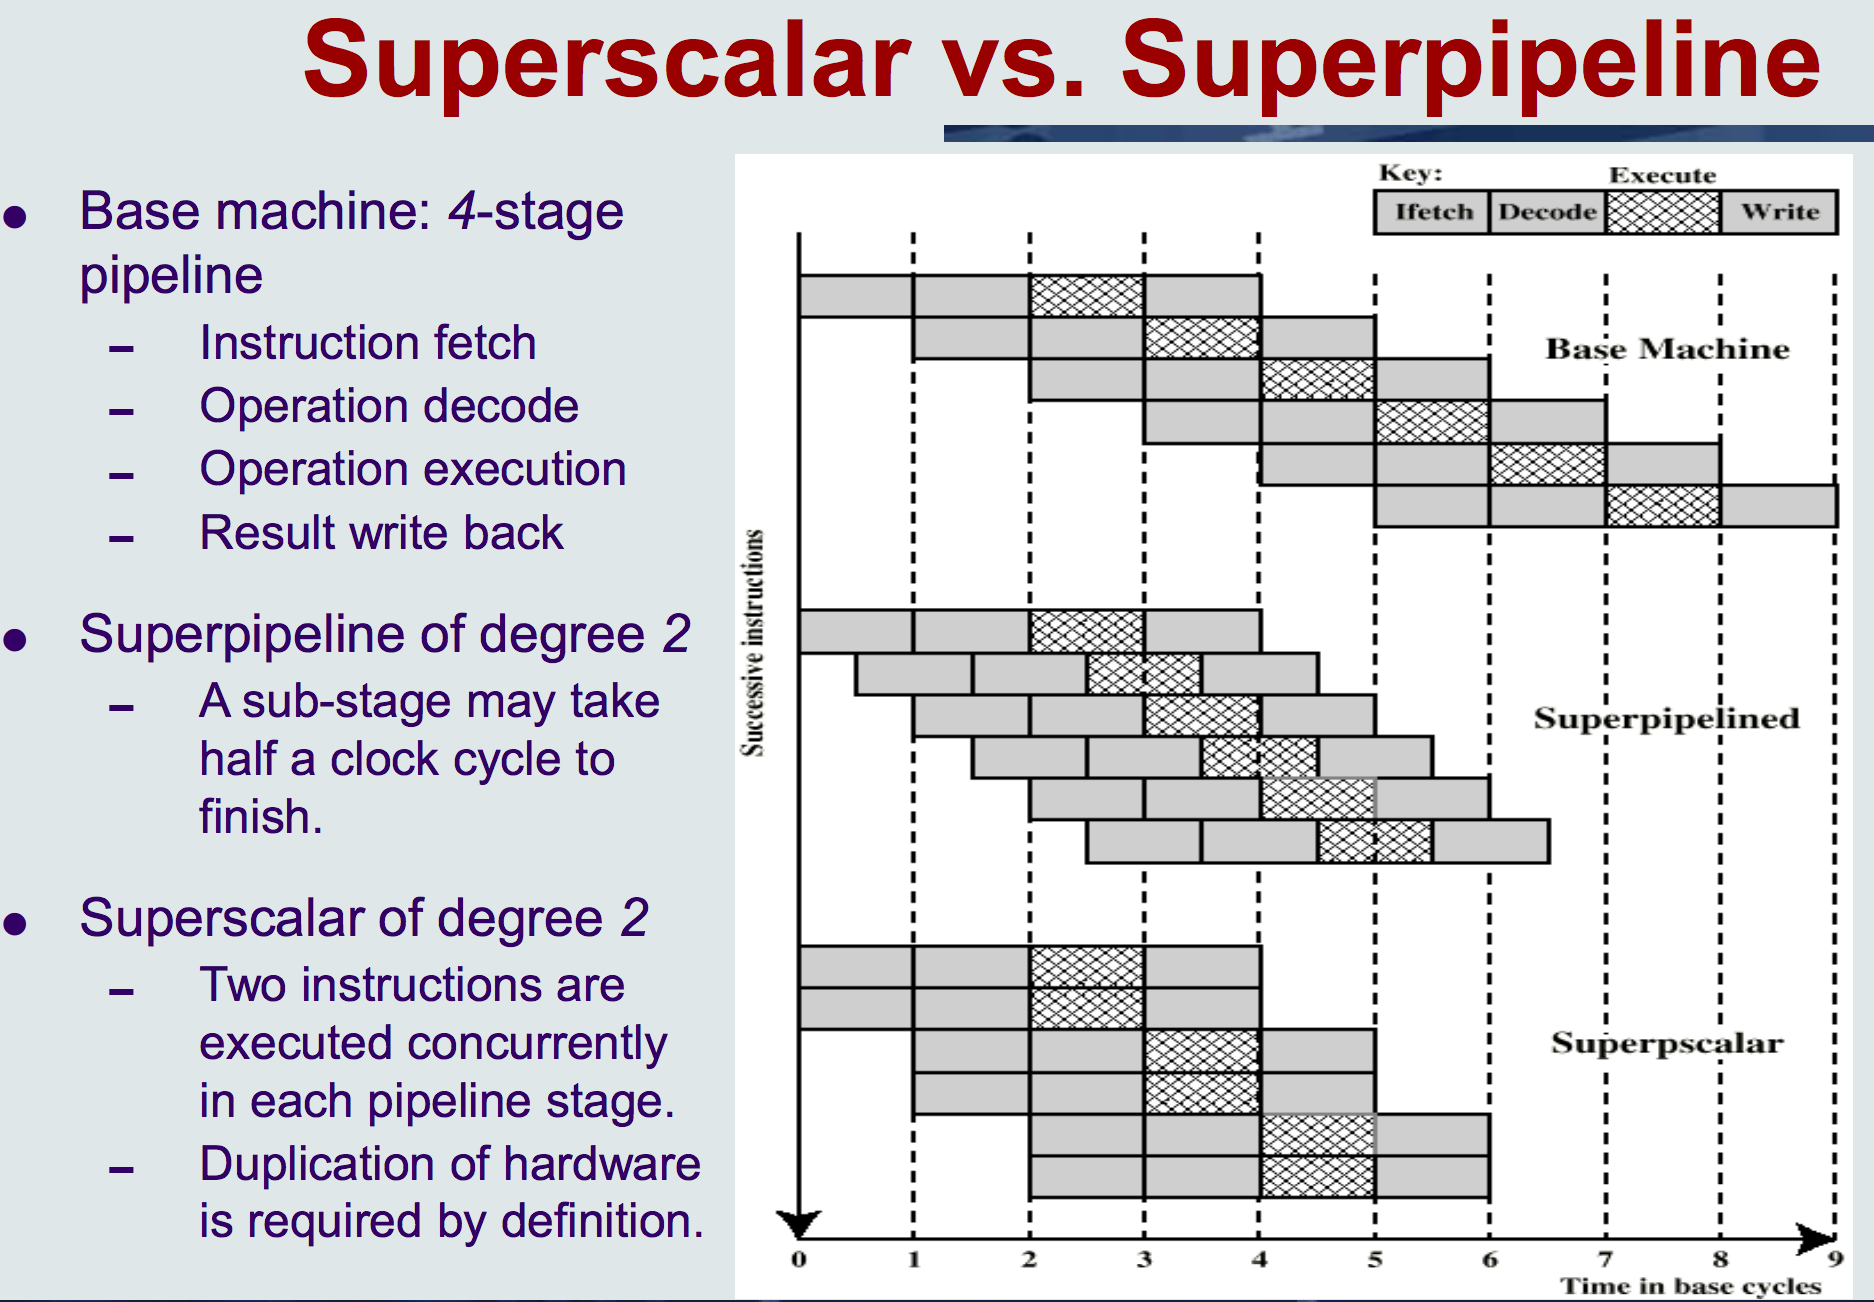
\includegraphics{img/superscalar-vs-superpipeline.png}}
  \caption{Difference between a Superscalar and a Superpipeline architecture}
  \label{fig:superscalar-vs-superpipeline}
\end{figure}


\subsection{Superscalar Superpipeline Design}

\begin{figure}[H]
  \centering
  \scalebox{0.342}{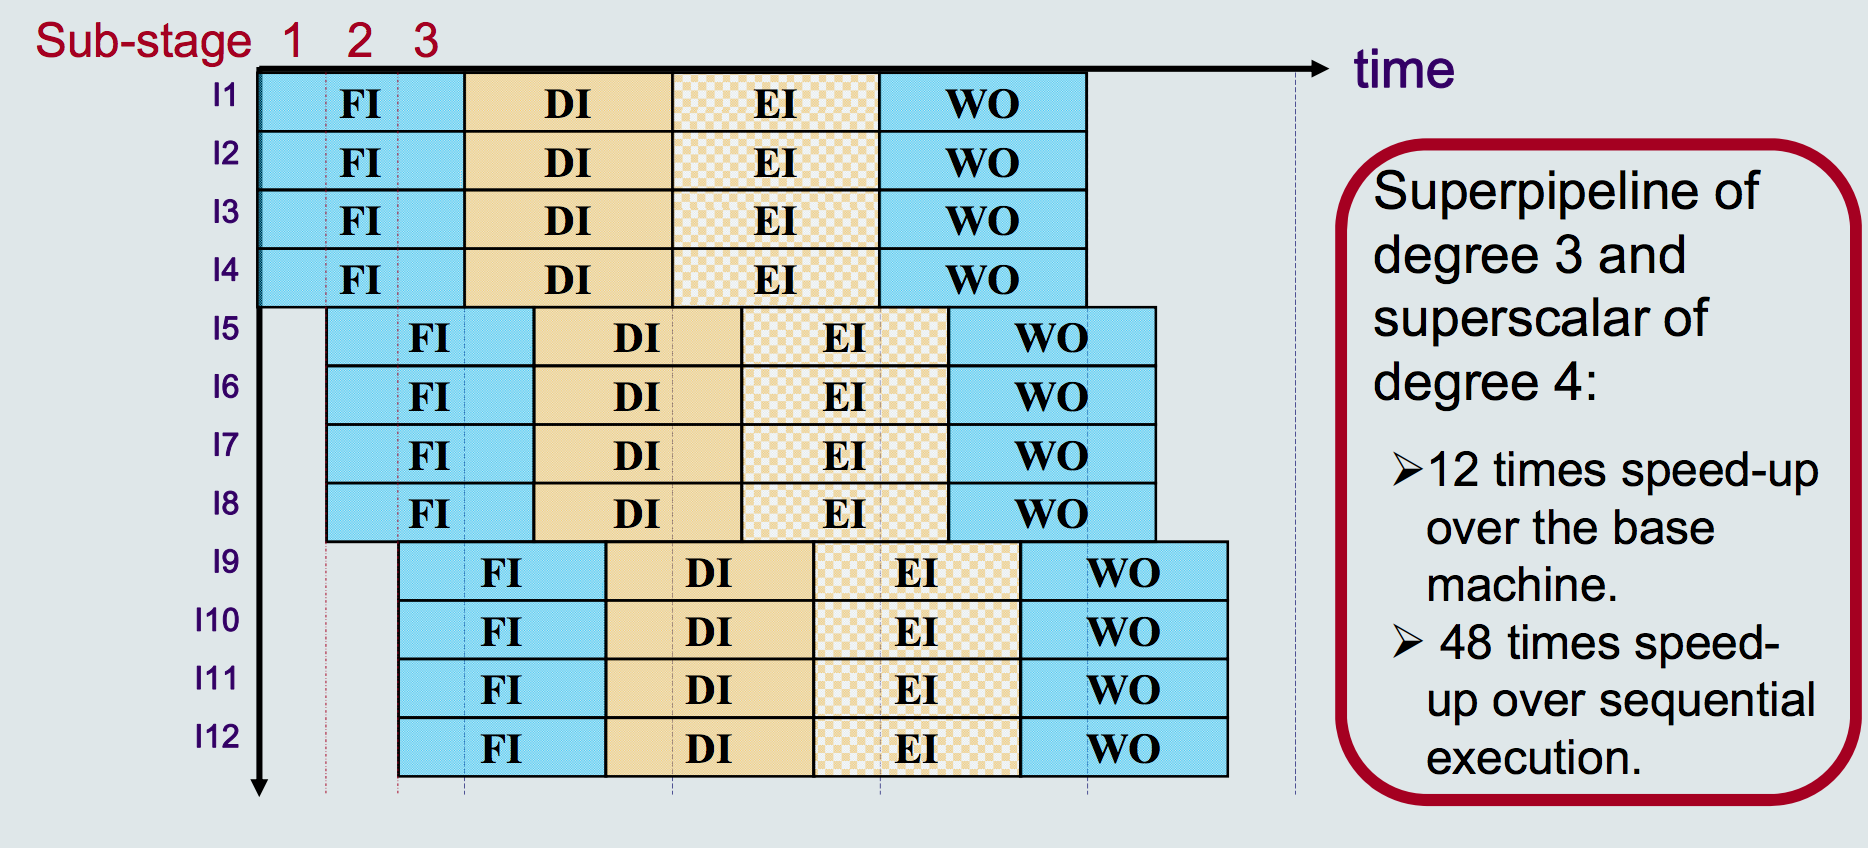
\includegraphics{img/superscalar-superpipeline.png}}
  \caption{Superscalar Superpipeline architecture}
  \label{fig:superscalar-superpipeline}
\end{figure}

The new trend is to combined the two ideas. In Figure \ref{fig:superscalar-superpipeline} it says that this would give us a 48 times speedup, this is not the case though because of data dependencies.

\subsection{Dependency issues}
The main problems are:
-- Resource conflicts. \\
-- Control (procedural) dependency. \\
-- Data dependencies. \\

These are very similar to the cases in normal pipelining (data hazards). But the consequences are more severe here because the parallelism are greater and thus larger amount of performance will be lost. \\

\subsubsection{Resource Conflicts}
Several instructions compete for the same hardware resource at the same time.
-- For instance, two aritmethic instructions need the same floating-point unit for execution. \\
-- similar to structural hazards in pipeline. \\

They can be solved \underline{partly} by introducing several hardware units for the same functions. \\
-- e.g. have two floating point units. \\
-- the hardware units can also be pipelined to support several operations at the same time. \\
-- however, memory units \textbf{can't be duplicated}.

\subsubsection{Procedural Dependency}

\subsubsection{Data Conflicts}

\subsubsection{Window of execution}

\subsubsection{Data Dependency}

\subsubsection{True Data Dependency}

\subsubsection{Output Dependency}

\subsubsection{Anti Dependency}

\subsubsection{Effect of Dependencies}

\subsection{Parallel instruction execution}

\subsubsection{Instruction vs Machine Parallelism}

\subsubsection{Division and Decoupling}

\subsubsection{SSA instruction Execution Policies}

\subsubsection{In-Order with In-Order Completion}
This seems important to understand

\subsubsection{In-Order issue with Out-of-Order Completion}
This seems important to understand

\section{Lecture 6: VLIW Processors}
The difference from Superscalar is that in that architecture the hardware solves everything for us, if improvements are made on the design we don't need to change the programs. \\
The down side though is that the architecture is very complex. \\
-- A lot of hardware is needed for run-time detection of parallelism. \\
-- It consumes a lot of power. \\
-- There is, therefore a limit in how far we can go with this technique. \\

The instruction window for execution is limited in size. \\
-- This limits the capacity to detect large number of parallel instructions.

\subsection{Very Long Instruction Word Processors}
Several operations that can be executed in parallel are placed in a single instruction word. \\
--VLIW rely on compile-time detecton of parallelism. \\
-- The compiler analyzes the program and detects operations to be executed in parallel. \\

After one instruction has been fetched, all the corresponding operations are issued in paralell.
The instruction window limitation disappears: the compiler can potentially analyze the whole program to detect parallel operations.

\subsubsection{Explicit Parallelism}
Instruction parallelism scheduled at compile time.\\
-- Included within the machine instructions explicitly.\\

An EPIC (Explicitly Parallel Instruction Computing) processor \\
--uses this information to perform parallel execution. \\

The hardware is very much simplified \\
-- The controller is similar to a simple scalar computer. \\
-- The number of FUs can be increased without needing additional sophisticated hardware to detect parallelism, as in SSA. \\

Compiler has much more time to determine parallel operations. \\
-- This analysis is only done once off-line, while run-time detection is carried out by SSA hardware for each execution of the code. \\
--Good compilers can detect parallelism based on global analysis of the whole program. \\

\subsubsection{Main issues}
-- Need a large number of registers. \\
-- Large data transport capacity is needed between Fus and the register files and between register files and memory. \\
-- High bandwidth between instruction cache and fetch unit is also needed due to long iunstructions.

\subsubsection{Software issues}

\subsection{Loop unrolling}

\subsection{IA-64 architecture}
\subsubsection{Predicated execution}
\subsubsection{Instruction format}
\subsubsection{Branch Predication}
\textbf{NOT THE SAME AS BRANCH PREDICTION}
\subsubsection{Placement of Loading}
\subsubsection{Speculative Loading}

\section{Parallel Processing}
\subsubsection{Why Parallel Processing?}
\subsubsection{Parallel Computer}
\subsubsection{Parallel Program}

\subsection{Architecture classification}
\subsubsection{Flynn’s Classification of Architectures}
-- Single instruction, single data stream - \textbf{SISD} \\
-- Single instruction, multiple data stream - \textbf{SIMD} \\
-- Multiple instruction, single data stream - \textbf{MISD} \\
-- Multiple instruction, multiple data stream- \textbf{MIMD} \\

\todo{GÅ IGENOM DESSA}\\

\subsection{Performance evaluation}

\subsection{Interconnection network}
\subsubsection{Single Bus}
\subsubsection{Completely Connected Network}
\subsubsection{Crossbar Network}
\subsubsection{Mesh Network}
\subsubsection{Hypercube Network}

\section{Lecture 8: SIMD Architectures}

\subsection{Vector Processors}
-- array processors \\
-- vector processors \\
-- data parallelism \\
Typical SISD processors who behave like SIMD processors

\subsubsection{Instruction-level parallelism}
\subsubsection{Thread-level parallelism}
\subsubsection{Data parallelism}
\subsubsection{Vector Processors}
\subsection{Array Processors}
Typical SIMD processors

\subsection{Dedicated Memory Organization}
\subsection{Global Memory Organization}
\subsection{Cray supercomputers}
\subsubsection{Cray X1}
\subsection{Multimedia extensions}
\subsubsection{sub-word execution}
\subsubsection{Packed Data Types}
\subsubsection{SIMD Arithmetic Examples}

\section{Lecture 9: MIMD Architectures}
A set of general purpose processors connected together \\
In contrast to a SIMD computer, a MIMD computer can execute different programs on different processors. \\

-- Works asynchronously, and don't have to synchronize with each other. \\
-- At any time, different processors may be executing different instructions on different pieces of data. \\
-- They can be built from commodity (off-the-shelf) microprocessors with relatively little effort. \\
-- They are also highly scalable, provided that an appropiate memory organization is used. \\
-- Most current parallel computer are built based on the MIMD architecture. \\

\subsubsection{SIMD vs. MIMD}
\subsubsection{MIMD Processor Classification}
\subsubsection{MIMD with Shared Memory}
\subsubsection{MIMD with Distributed Memory}
\subsubsection{Shared-Address-Space Platforms}
\subsubsection{Multi-Computer Systems}
\subsubsection{MIM Design Issues}
\subsection{Symmetric multiprocessors (SMP)}
\subsubsection{SMP Advantages}
\subsubsection{SMP based on Shared Bus}
\subsubsection{Multi-Port Memory SMP}
\subsubsection{Operation System Issues}
\subsubsection{IBM S/390}
\subsection{NUMA Architecture}
\subsubsection{Memory Access Approaches}
\subsection{Clusters}
\subsubsection{Losely Coupled MIMD - Clusters}
\subsubsection{Clusters benefits}
\subsubsection{Clusters Configurations}
\subsubsection{IBM Blue Gene Supercomputer}
\subsubsection{Parallelizing Computation}
\subsubsection{Google Applications}

\section{Lecture 10: Cache Coherence}
To many section without text seems to bug \LaTeX
\subsection{Introduction}
\subsubsection{Write Through}
\subsubsection{Write Back}
\subsubsection{Software Solutions}
\subsubsection{Hardware Solutions}
\subsection{Directory protocols}
\subsubsection{Cache Coherence Operations}
\subsection{Snoopy protocols}
\subsubsection{Write Invalidate SP}
\subsubsection{Snoopy Cache Organization}
\subsubsection{MESI State Transition Diagram}
\subsubsection{Write Update SP}
\subsubsection{Invalidate vs. Update Protocols}
\subsubsection{Directory vs. Snoopy Schemes}
\subsection{L1-L2 consistence}
\subsubsection{Alpha-Server 4100}

\section{Lecture 11: Multi-Core and GPU}
To many section without text seems to bug \LaTeX
\subsection{Multi-Core Computers}
\subsubsection{Intel Core i7}
\subsubsection{Superscalar vs. Multi-Core}
\subsubsection{Single Core vs. Multi-Core}
\subsubsection{Intel Polaris}
\subsection{Multithreading}
\subsubsection{Thread-Level Parallelism (TLP)}
\subsubsection{Scalar Processor Approaches}
\subsubsection{Superscalar Approaches}
\subsubsection{SMT and Chip Multiprocessing}
\subsubsection{Multithreading Paradigms}
\subsection{Graphic Processing Unit (GPU)}
\subsubsection{CPU vs. GPU}
\subsection{General Purpose GPUs}
\subsubsection{Divergent Execution}
\subsubsection{Reduce Branch Divergence}
\subsubsection{GPUPU}
\subsubsection{NVIDIA Tesla}
\subsubsection{CUDA Programming Language}

\end{document}

